\documentclass[11pt]{article}

\title{TCR Clustering Experiments}

\author{Max Van Houcke}
\date{}

% Packages
\usepackage{amsmath}
\usepackage{graphicx}
\usepackage{float}

% Document
\begin{document}

    \maketitle

    \section{Z Scores}

    Trying out z\_scores to vectorize the sequences

    \begin{figure}[H]
        \makebox[\textwidth]{
            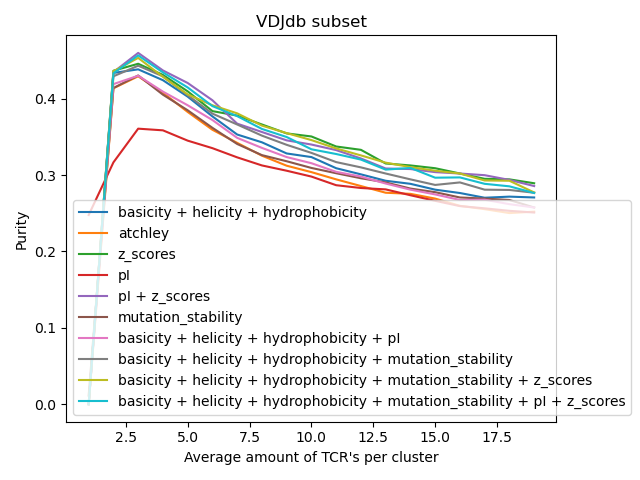
\includegraphics[width=0.49\textwidth]{img/z_scores_purity.png}
            \hfill
            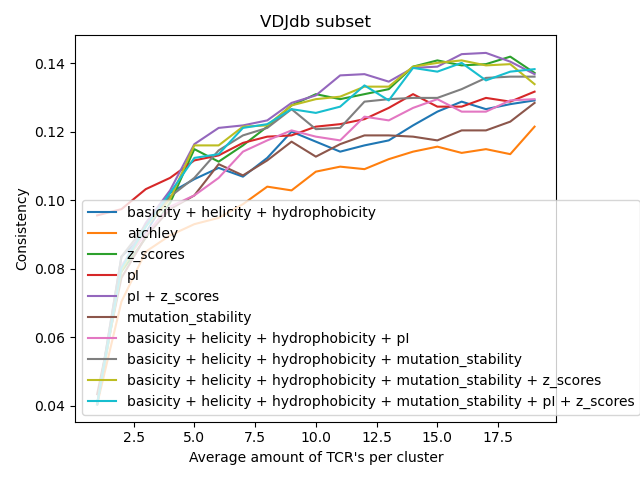
\includegraphics[width=0.49\textwidth]{img/z_scores_consistency.png}
        }
    \end{figure}

    Results are very pleasing, so we focus on some more combinations with the z\_scores

    \begin{figure}[H]
        \makebox[\textwidth]{
            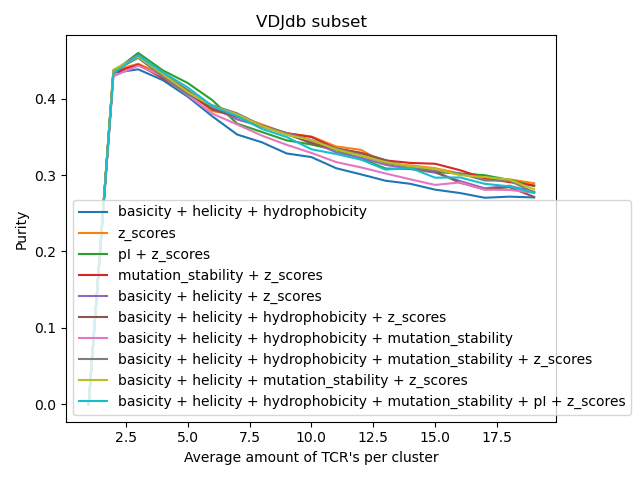
\includegraphics[width=0.49\textwidth]{img/z_scores_purity_more.png}
            \hfill
            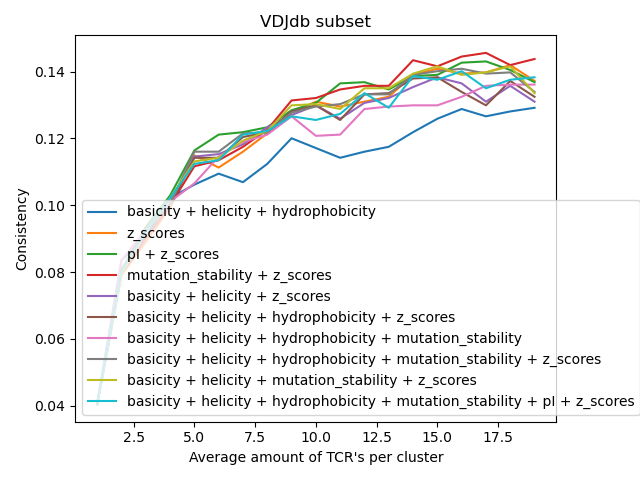
\includegraphics[width=0.49\textwidth]{img/z_scores_consistency_more.png}
        }
    \end{figure}

    The combination of the z\_scores with mutation stability seems to be a winner.

    \section{Manually weighting the vectors}

    By manually applying a low factor to the sides of the vectors, we try to give more
    importance to the central amino acids, in the hope of a better clustering.

    \begin{center}
        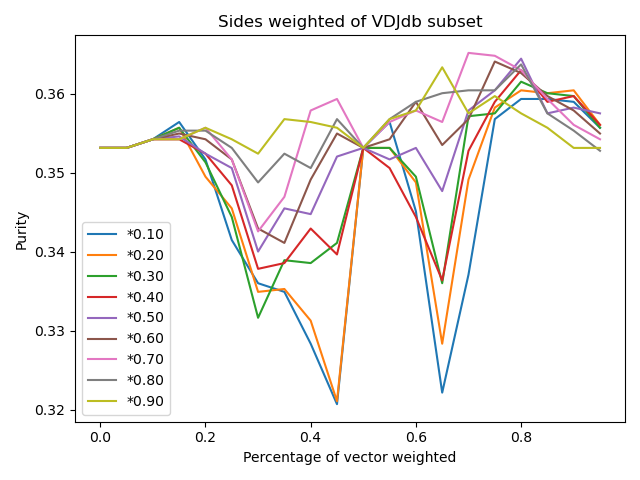
\includegraphics[width=0.8\linewidth]{img/weighting_manually.png}
    \end{center}

    It seems that, in general, applying a weight to a large part of the vector (around 70 to 80 percent) and thus giving more
    importance to only the most central amino acids gives the biggest advantage.
    This in combination with a not too drastic factor.

    Applying more drastic factors to the vector only works when weighting a very large ( $> 80\%$) percent of the vector.
    A significant dip in purity happens otherwise, as can be seen on the graph.

    \subsection{Corrections}

    As Pieter pointed out, there is an inflection point at x 0.5 in the manual weighting graphs.
    I revisited the code and found that at 0.5 the whole vector is already weighted.
    This brings up the question why better results are achieved after 0.5.
    The code wrapped around and actually started weighting the center amino acid.
    Therefore I experiment with both weighting methods and run them on the whole VDJdb as well instead of only on the
    subset.

    \subsubsection{Sides weighted}

    \begin{figure}[H]
        \makebox[\textwidth]{
            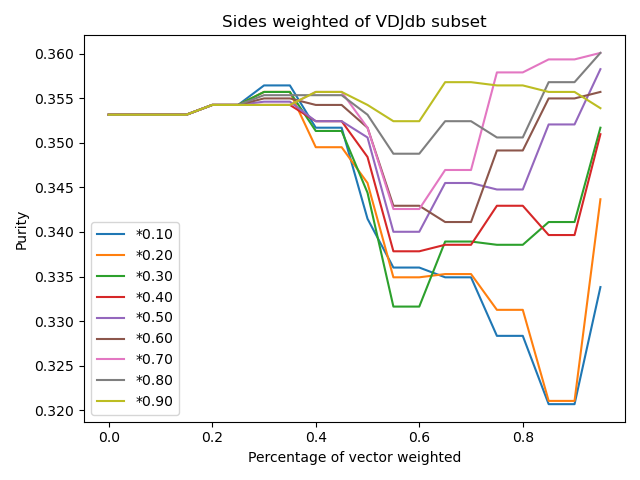
\includegraphics[width=0.49\textwidth]{img/sides_vdjsubset_purity.png}
            \hfill
            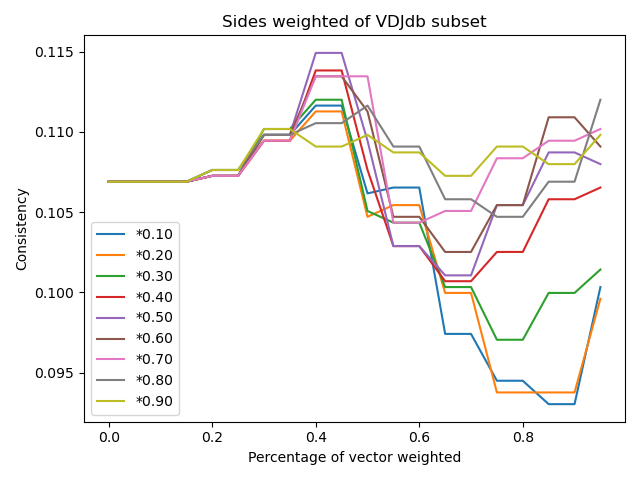
\includegraphics[width=0.49\textwidth]{img/sides_vdjsubset_consistency.png}
        }
        \makebox[\textwidth]{
            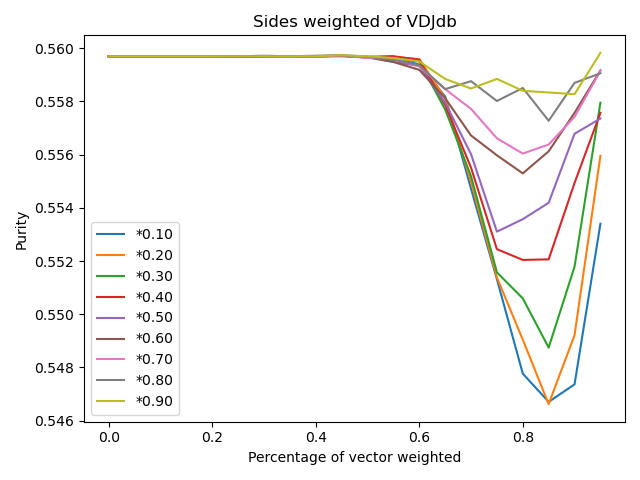
\includegraphics[width=0.49\textwidth]{img/sides_vdj_purity.png}
            \hfill
            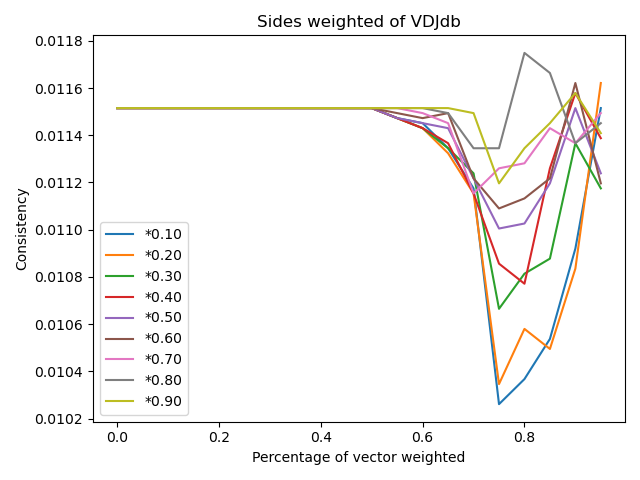
\includegraphics[width=0.49\textwidth]{img/sides_vdj_consistency.png}
        }
    \end{figure}

    \subsubsection{Center weighted}

    \begin{figure}[H]
        \makebox[\textwidth]{
            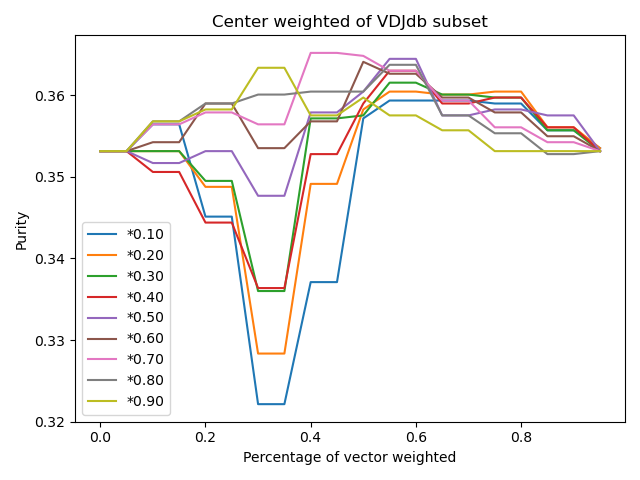
\includegraphics[width=0.49\textwidth]{img/center_vdjsubset_purity.png}
            \hfill
            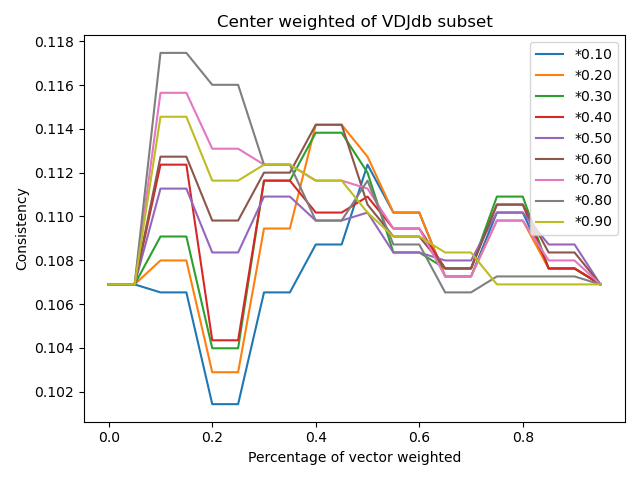
\includegraphics[width=0.49\textwidth]{img/center_vdjsubset_consistency.png}
        }
        \makebox[\textwidth]{
            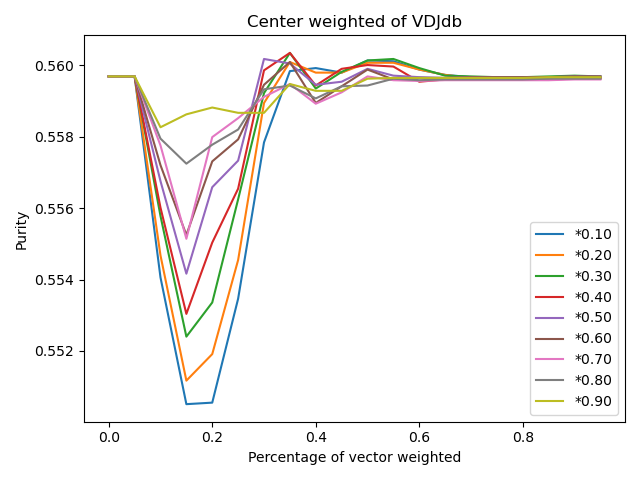
\includegraphics[width=0.49\textwidth]{img/center_vdj_purity.png}
            \hfill
            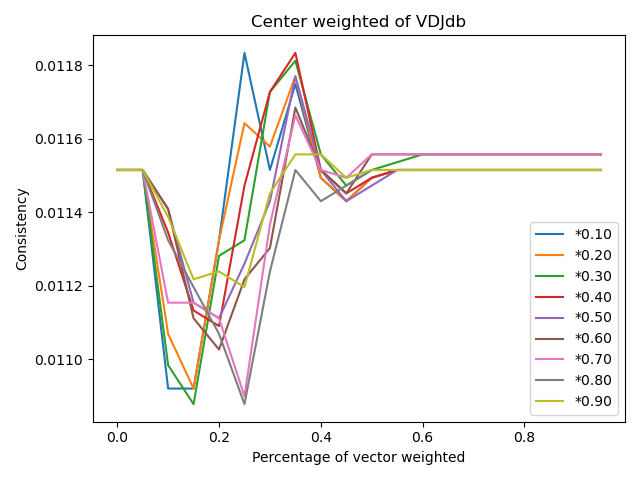
\includegraphics[width=0.49\textwidth]{img/center_vdj_consistency.png}
        }
    \end{figure}

    \subsubsection{Remarks}

    It seems that, against the theory that the central amino acids are more important, weighting the central amino acids
    and thus giving more importance to the sides of the vector.
    This is both the case for the subset as well as as the full VDJdb.

    \subsection{More corrections}

    The weird conclusion of having better results with more importance to the sides, was unexpected.
    This brings up the question if there any any faults in the code.
    A possible explanation, given by Pieter, was having the vector padded before applying the weights.
    This was indeed the case.
    After correcting this we get the following graphs.

    \begin{figure}[H]
        \makebox[\textwidth]{
            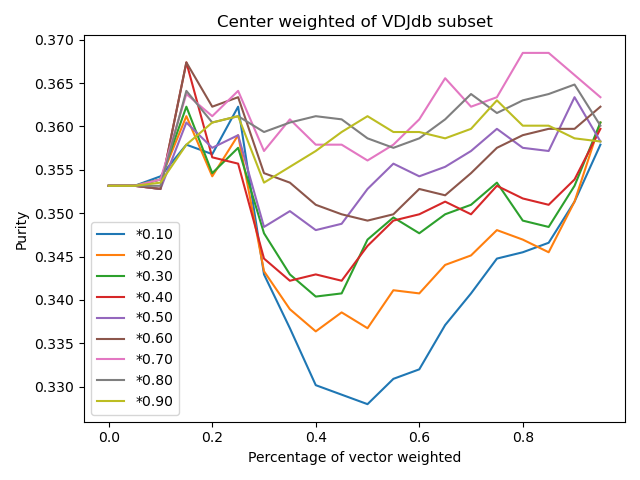
\includegraphics[width=0.49\textwidth]{img/center_vdjsubset_purity_corr.png}
            \hfill
            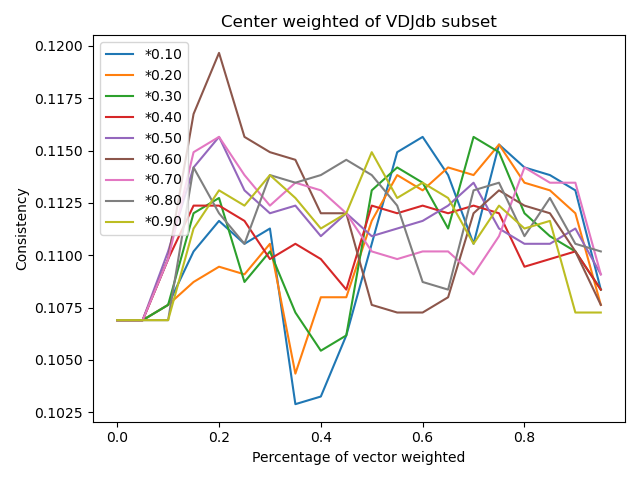
\includegraphics[width=0.49\textwidth]{img/center_vdjsubset_consistency_corr.png}
        }
        \makebox[\textwidth]{
            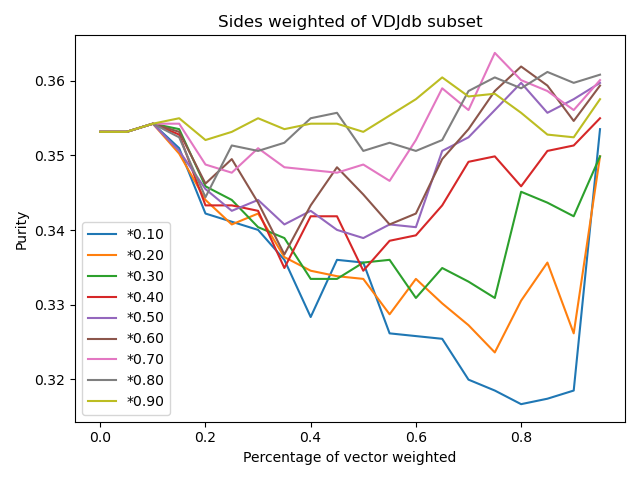
\includegraphics[width=0.49\textwidth]{img/sides_vdjsubset_purity_corr.png}
            \hfill
            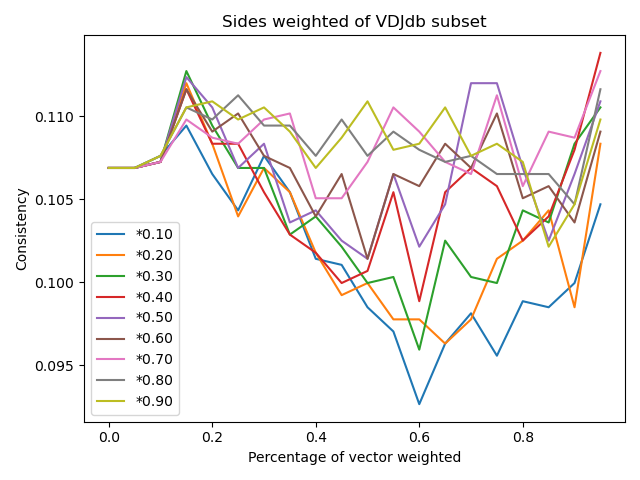
\includegraphics[width=0.49\textwidth]{img/sides_vdjsubset_consistency_corr.png}
        }
    \end{figure}

    \section{Finding pairs with a small distance}

    To integrate the project into Sebastiaan's research, the first step we try is finding pairs close to each other using
    faiss.

    By finding these pairs and then calculating the distance between them, we can make an approximation of a distance matrix
    much quicker than doing it manually.

    The way we approach this is by generating large clusters and calculating the distance for each possible pair in every cluster.
    To evaluate this method, we compare the pairs found with a distance of 1 against the pairs found with the hashing method from Pieter, which
    finds all pairs with a distance of 1 quickly in a dataset.

    For our clustering approach, we should determine how large the clusters are that we generate.
    Intuitively, larger clusters will mean larger computation time, as the distance for each possible pair in every cluster is calculated.
    However, larger clusters will also mean higher accuracy, as the chance of finding pairs that are close to each other is higher.

    We plot a couple of different cluster sizes and their accuracy:

    \begin{figure}[H]
        \centering
        \begin{minipage}{0.45\textwidth}
            \centering
            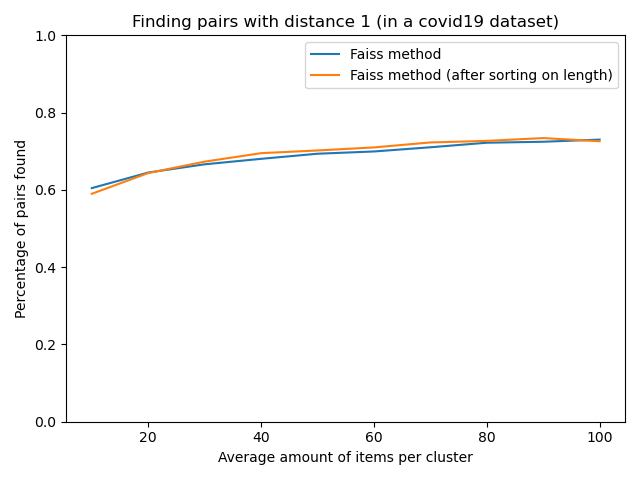
\includegraphics[width=0.9\textwidth]{img/pairs1_covid19.png}
            \caption{Dataset of 27000 sequences}
        \end{minipage}\hfill
        \begin{minipage}{0.45\textwidth}
            \centering
            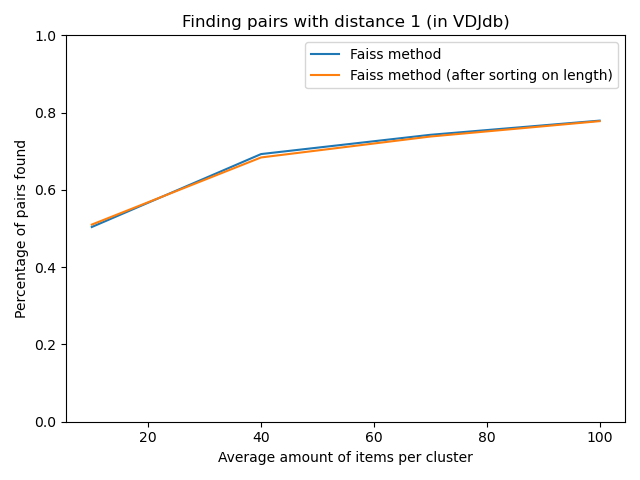
\includegraphics[width=0.9\textwidth]{img/pairs1_vdj.png}
            \caption{VDJdb dataset of 47000 sequences}
        \end{minipage}
    \end{figure}

    For reference, distance calculation for the VDJdb with average 90 sequences per cluster took around 18 seconds.


\end{document}